% ----------------------------------------------------------
\chapter{Desenvolvimento e Análise dos Resultados Obtidos}\label{cap:desenvolvimento_e_analise_resultados}
% ----------------------------------------------------------
Este capítulo apresenta o processo de desenvolvimento do projeto de fim de curso relativo ao desenvolvimento de um sistema de gerenciamento de reservas e controle automatizado de dispositivos IoT para quadras esportivas. Na \autoref{sec:ferramentas_tecnologias} são apresentadas as ferramentas e tecnologias utilizadas no desenvolvimento do sistema. A \autoref{sec:desenvolvimento} apresenta o processo de desenvolvimento do PFC e a \autoref{sec:analise_resultados} dispõe dos resultados alcançados ao fim do processo.

% \textbf{Instruções da Coordenação do PFC:}

% Neste capítulo, deve-se:
% \begin{itemize}
% 	\item Descrever detalhadamente como foi feita a implementação/desenvolvimento da solução proposta;
% 	\item Deixar bem claro e justificar tecnicamente para o leitor como que o desenvolvimento realizado implementa de fato a solução proposta, explicando tecnicamente as decisões que foram tomadas para se chegar a tal implentação;
% 	\item Analisar os resultados obtidos com base em indicadores, gráficos, estatísticas, etc: 
% 	\begin{itemize}
% 		\item A implementação realizada solucionou de fato o problema tratado? 
% 		\item Obteve-se o resultado esperado? 
% 		\item Mostrou-se melhor que o método anterior?
% 		\item Vantagens e desvantagens; 
% 		\item Problemas encontrados;   
% 		\item Impacto dos resultados obtidos nos processos/projetos/produtos/serviços/clientes da empresa/instituto de pesquisa; 
% 		\item Impactos organizacionais, tecnológicos, financeiros, éticos, ecológicos, etc.
% 	\end{itemize}
% \end{itemize}

% Sugere-se colocar uma diagrama/fluxograma ilustrando como que a solução proposta foi implementada/desenvolvida, e depois explicar em detalhes cada parte/bloco do diagrama/fluxograma ao longo do texto. 

% Ressaltamos que, em princípio, existe uma infinidade de maneiras diferentes de implementar a solução proposta. Desse modo, o diagrama/fluxograma da solução proposta apresentado no capítulo anterior é mais geral e abstrato que o diagrama/fluxograma da implementação: a implementação realizada no PFC é uma maneira específica de se chegar à solução proposta a partir das técnicas, ferramentas e métodos utilizados. 

Alguns pontos que serão explicados nesse capítulo:

\begin{itemize}
	\item \textbf{Ferramentas}: As tecnologias utilizadas na implementação da solução proposta, como linguagens de programação, frameworks, bibliotecas, etc.
	\item \textbf{Arquitetura da solução}: A arquitetura utilizada na implementação da solução proposta, como monolítica, microsserviços, cliente-servidor, etc.
	\item \textbf{Modelagem do banco de dados}: O modelo utilizado para representar os dados da aplicação, incluindo as entidades, relacionamentos, atributos, etc.
	\item \textbf{Backend}: A parte da solução que lida com a manipulação dos dados e a regra de negócio da aplicação.
	\subitem{\textbf{Registro e autenticação de usuários}: Como o backend implementa a funcionalidade de registro e autenticação de usuários, incluindo validações, segurança, etc.}
	\subitem{\textbf{Autorização de usuários}: Como o backend implementa a funcionalidade de autorização de usuários, incluindo permissões, roles, etc.}
	\subitem{\textbf{Rotas da aplicação}: Como o backend implementa as rotas da aplicação, incluindo endpoints de CRUD para tenanants, quadras, agendamentos de horários e credenciais de acesso a API relacionada à internet das coisas (IoT).}
	\subitem{\textbf{Detalhamento do agendamentos de horários}: Como o backend implementa a funcionalidade de agendamentos de horários de quadras, incluindo informações sobre os locais, os tipos de atividades, as datas e as horas.}
	\subitem{\textbf{Detalhamento da integração com IoT}: Como o backend implementa a integração com dispositivos IoT e comanda o acionamento e desligamento de acordo com os agendamentos feitos pelosus usuários.}
	\item \textbf{Análise de resultados}: Análise dos resultados obtidos com o desenvolvimento da aplicação. Detalhando os principais aspesctos relevantes, como a eficiência do agendamento de horários, a segurança das informações e a integração com IoT.
\end{itemize}

\section{Ferramentas e Tecnologias Utilizadas}\label{sec:ferramentas_tecnologias}

A seção de ferramentas e tecnologias utilizadas no desenvolvimento deste projeto apresenta um panorama detalhado dos recursos técnicos empregados para a construção da aplicação de servidor do sistema de gerenciamento de reservas e controle automatizado de dispositivos IoT para quadras esportivas. 
% O projeto foi desenvolvido utilizando uma stack moderna e robusta, com o backend implementado em Nest.js, um framework eficiente e escalável para Node.js, e o frontend será desenvolvido em React, a fim de proporcionar uma experiência de usuário dinâmica e responsiva. Além disso, o banco de dados relacional PostgreSQL foi utilizado para garantir a integridade e a consistência dos dados, enquanto a integração com a plataforma eWeLink permitiu o controle automatizado de dispositivos IoT, agregando um nível adicional de automação e inovação ao sistema. Este conjunto de ferramentas foi escolhido com o objetivo de garantir um desenvolvimento ágil, eficiente e que atendesse às necessidades específicas do projeto.

\subsection{Git}

O Git é um sistema de controle de versão distribuído criado por Linus Torvalds em 2005, inicialmente para o desenvolvimento do kernel do Linux. Antes do Git, o projeto Linux utilizava o BitKeeper, mas devido a restrições de licenciamento, Torvalds decidiu desenvolver uma ferramenta própria. O objetivo principal era criar um sistema rápido, eficiente e que suportasse grandes projetos com facilidade.

As principais funções do Git incluem rastreamento de alterações no código-fonte, permitindo que múltiplos desenvolvedores trabalhem simultaneamente em um mesmo projeto sem conflitos. O Git possibilita a criação de ramificações (branches) para desenvolver novos recursos ou corrigir bugs de forma isolada, facilitando a integração dessas alterações ao projeto principal posteriormente. Além disso, como um sistema distribuído, cada desenvolvedor possui uma cópia completa do repositório, o que aumenta a segurança e a integridade dos dados. Atualmente, o Git é a ferramenta de controle de versão mais popular do mundo, amplamente utilizada por empresas de software, desenvolvedores independentes e projetos de código aberto.

Decidiu-se utilizar o Git devido a familiaridade da equipe com a ferramenta, já que é amplamente usada em outros projetos na empresa, além de sua robustez e confiabilidade.
 
O Git revolucionou a forma como o desenvolvimento de software é conduzido, proporcionando uma maneira eficiente e colaborativa de gerenciar projetos complexos. Sua flexibilidade, velocidade e robustez tornaram-no uma ferramenta essencial no arsenal de qualquer desenvolvedor, suportando desde pequenos projetos individuais até grandes sistemas empresariais.

\subsection{GitHub}

O GitHub é uma plataforma de hospedagem e repositório de código-fonte e arquivos que utiliza o Git para controle de versão. A plataforma permite que programadores ou qualquer usuário cadastrado contribuam em projetos, sejam eles privados ou de código aberto, de qualquer lugar do mundo. Amplamente adotada por desenvolvedores, o GitHub facilita a divulgação de trabalhos e a colaboração em projetos, além de oferecer recursos que simplificam a comunicação, como a identificação de problemas e a mesclagem de repositórios remotos por meio de issues e pull requests.

Atualmente, o GitHub é utilizado globalmente, contando com mais de 36 milhões de usuários ativos que contribuem em projetos comerciais ou pessoais. A plataforma hospeda mais de 100 milhões de projetos, incluindo alguns de renome mundial, como WordPress, GNU/Linux, Atom e Electron. Além disso, o GitHub oferece suporte a recursos de organização, amplamente utilizados por aqueles que desejam expandir seus projetos.

O Github é uma ferramenta usada por padrão na Fischertec. Embora outras plataformas como o Gitlab tenham funções semelhantes, optou-se por manter o padrão da empresa.

\subsection{PostgreSQL}

O SQL (Structured Query Language) foi desenvolvido nos anos 1970 pela IBM como uma linguagem padrão para gerenciar e manipular bancos de dados relacionais. PostgreSQL, um sistema de gerenciamento de banco de dados relacional, surgiu na Universidade da Califórnia em Berkeley, no final dos anos 1980, como parte do projeto POSTGRES (Post Ingres). Em 1996, o sistema foi renomeado para PostgreSQL, refletindo sua compatibilidade com SQL. Desde então, PostgreSQL evoluiu significativamente, tornando-se uma das bases de dados relacionais mais robustas e avançadas disponíveis.

PostgreSQL oferece uma ampla gama de funções, incluindo suporte a transações ACID (Atomicidade, Consistência, Isolamento, Durabilidade), integridade referencial, e extensões para manipulação de dados complexos como JSON e XML. Além disso, suporta procedimentos armazenados, gatilhos e uma variedade de tipos de índices para otimizar consultas. Atualmente, PostgreSQL é amplamente utilizado por grandes empresas, startups e projetos de código aberto devido à sua confiabilidade, flexibilidade e conformidade com os padrões SQL.

Existem outras soluções de banco de dados SQL como MySQL, que é conhecido por sua facilidade de uso e performance em aplicações web, e soluções NoSQL como MongoDB, que é ideal para armazenar grandes volumes de dados não estruturados e aplicações que exigem alta escalabilidade e flexibilidade. Optou-se por usar o PostgreSQL no desenvolvimento do projeto devido à sua capacidade de lidar com transações complexas, suporte a dados estruturados e não estruturados, e forte conformidade com os padrões SQL, o que garante integridade e consistência dos dados.

O PostgreSQL se destaca como uma solução de banco de dados robusta e versátil, adequada para uma ampla gama de aplicações. Sua evolução ao longo dos anos e a capacidade de suportar funcionalidades avançadas o tornam uma escolha excelente para projetos que exigem confiabilidade e flexibilidade. A decisão de utilizá-lo no projeto foi fundamentada em sua capacidade de atender às necessidades específicas de gerenciamento de dados de maneira eficiente e segura.

\subsection{Typescript}

O JavaScript, criado em 1995 por Brendan Eich da Netscape, rapidamente se tornou a linguagem padrão para desenvolvimento web, permitindo a criação de páginas dinâmicas e interativas. No entanto, à medida que aplicações web se tornavam mais complexas, as limitações de JavaScript em termos de tipagem estática e suporte para grandes projetos se tornaram evidentes. Para reduzir essas limitações, a Microsoft lançou o TypeScript em 2012, uma linguagem de programação de código aberto que é um superconjunto (superset) estrito de JavaScript. TypeScript adiciona tipagem estática e outros recursos avançados ao JavaScript, ajudando os desenvolvedores a escrever código mais seguro e escalável.

As principais funções do TypeScript incluem a adição de tipos estáticos, interfaces, classes e módulos, que não existem nativamente no JavaScript. Essas funcionalidades permitem a detecção de erros durante o desenvolvimento, antes do tempo de execução, melhorando a qualidade do código. Além disso, TypeScript se transpila (é convertido) para JavaScript, garantindo compatibilidade total com os navegadores e plataformas que suportam JavaScript. Atualmente, TypeScript é amplamente adotado em projetos de grande escala devido à sua capacidade de melhorar a produtividade e a manutenção do código. Empresas como Google, Microsoft e Airbnb utilizam TypeScript em seus projetos.

No desenvolvimento do projeto backend, optou-se por TypeScript em vez de JavaScript por várias razões. TypeScript proporciona uma melhor experiência de desenvolvimento, oferecendo autocompletar, navegação de código e verificação de tipos em tempo de compilação, o que ajuda a evitar muitos erros comuns em JavaScript. Isso é especialmente importante em projetos backend, onde a robustez e a previsibilidade do código são cruciais. Além disso, TypeScript facilita a colaboração entre desenvolvedores, permitindo que eles entendam e mantenham o código com mais facilidade.

O TypeScript se destaca como uma ferramenta poderosa que complementa e aprimora JavaScript, tornando o desenvolvimento de software mais eficiente e menos propenso a erros. Sua adoção no desenvolvimento da aplicação backend de gerenciamento de reservas e controle automatizado de dispositivos IoT permitiu criar um código mais robusto e sustentável.

\subsection{Node.js}

O Node.js é uma plataforma de desenvolvimento open-source baseada no motor JavaScript V8 do Google Chrome, criada em 2009 por Ryan Dahl. Seu objetivo inicial era possibilitar a execução de JavaScript no lado do servidor, permitindo o desenvolvimento de aplicações web com maior eficiência e escalabilidade. Desde seu lançamento, o Node.js rapidamente ganhou popularidade devido à sua arquitetura orientada a eventos e sua capacidade de lidar com operações de entrada e saída de forma não bloqueante, o que é particularmente útil para aplicações em tempo real.

Atualmente, o Node.js é amplamente utilizado para construir desde APIs e microservices até aplicações completas de grande escala. Sua capacidade de executar JavaScript tanto no cliente quanto no servidor facilita o desenvolvimento fullstack, enquanto a vasta biblioteca de pacotes disponíveis através do npm (Node Package Manager) oferece soluções para praticamente qualquer necessidade de desenvolvimento. O Node.js tem sido uma escolha popular em diversas indústrias devido à sua performance, escalabilidade e ao suporte contínuo de uma grande comunidade de desenvolvedores.

Uma das principais vantagens do Node.js em comparação com outras soluções é sua natureza assíncrona e orientada a eventos, que permite o gerenciamento eficiente de múltiplas conexões simultâneas sem sobrecarregar os recursos do servidor. Além disso, a utilização de JavaScript, uma linguagem amplamente conhecida e utilizada, reduz a curva de aprendizado para novos desenvolvedores e facilita a integração entre equipes de frontend e backend. A modularidade do Node.js e sua grande comunidade de apoio também contribuem para o desenvolvimento mais rápido e eficiente de aplicações.

Portanto o Node.js se destaca como uma solução versátil e eficiente para o desenvolvimento de aplicações modernas. Sua combinação de performance, escalabilidade e uma vasta gama de ferramentas e bibliotecas tornam-no uma escolha robusta para desenvolvedores que buscam criar aplicações rápidas e escaláveis, atendendo às demandas de um mercado cada vez mais dinâmico e competitivo.

\subsection{Nest.js}

O Nest.js é um framework de desenvolvimento backend criado em 2017 por Kamil Myśliwiec. Inspirado nos princípios de programação modular e fortemente influenciado pelo Angular, o Nest.js foi projetado para oferecer uma estrutura robusta e escalável para a construção de aplicações do lado do servidor. Desde o seu lançamento, o framework tem crescido em popularidade, especialmente entre desenvolvedores que buscam uma abordagem moderna para o desenvolvimento de aplicações backend em Node.js.

O Nest.js fornece uma arquitetura modular que facilita a criação e a manutenção de aplicações escaláveis e bem estruturadas. Ele suporta diversos paradigmas de programação, incluindo orientação a objetos, programação funcional e reativa. Com suporte nativo para TypeScript, o Nest.js oferece tipagem estática, o que melhora a confiabilidade e a legibilidade do código. Atualmente, é amplamente utilizado para construir APIs RESTful, microservices e aplicativos monolíticos, sendo uma escolha frequente em projetos que exigem alta escalabilidade e flexibilidade.

Entre as principais vantagens do Nest.js estão sua modularidade, que permite a criação de aplicações altamente organizadas e de fácil manutenção, e seu suporte integral a TypeScript, que traz maior segurança e produtividade no desenvolvimento. Em comparação com outros frameworks, como Express.js, o Nest.js oferece uma estrutura mais robusta e orientada a boas práticas, facilitando o desenvolvimento de aplicações complexas. No contexto do projeto de fim de curso, o Nest.js foi escolhido por sua capacidade de suportar a criação de uma aplicação multi-tenant complexa, com necessidades específicas de escalabilidade, organização e integração com outras tecnologias.

O Nest.js se destaca como uma ferramenta poderosa para o desenvolvimento de aplicações backend modernas, combinando a performance do Node.js com uma arquitetura flexível e escalável. Sua adoção neste projeto de fim de curso reflete a busca por soluções eficientes e de alta qualidade, alinhadas com as demandas atuais do mercado de tecnologia.

\subsection{Docker}

O Docker foi lançado em 2013 por Solomon Hykes, inicialmente como um projeto interno da empresa dotCloud. A plataforma foi criada com o objetivo de simplificar o processo de desenvolvimento, distribuição e execução de aplicações por meio da virtualização de contêineres. Desde seu lançamento, o Docker tem revolucionado a maneira como aplicações são desenvolvidas e implantadas, tornando-se uma das ferramentas mais populares no ecossistema de DevOps.

Atualmente, o Docker é amplamente utilizado para criar, distribuir e executar aplicações em contêineres, que são ambientes leves e portáteis que contêm tudo o que uma aplicação precisa para ser executada. Isso inclui código, bibliotecas e dependências, garantindo que a aplicação funcione de maneira consistente em qualquer ambiente. O Docker é uma escolha comum em projetos que exigem portabilidade, escalabilidade e uma integração contínua eficiente, sendo adotado por empresas de todos os tamanhos para modernizar seus fluxos de trabalho de desenvolvimento e implantação.

Entre as principais vantagens do Docker estão a portabilidade de aplicações, a eficiência no uso de recursos e a facilidade de integração com pipelines de CI/CD (integração contínua e entrega contínua). Comparado com máquinas virtuais tradicionais, os contêineres do Docker são mais leves e rápidos, o que resulta em tempos de inicialização menores e melhor utilização de recursos. No contexto deste projeto, o Docker foi escolhido para garantir que o ambiente de desenvolvimento e produção seja consistente, facilitando a implantação em servidores AWS e reduzindo problemas de compatibilidade.

O Docker se destaca como uma solução essencial para o desenvolvimento e a implantação de aplicações modernas, oferecendo uma maneira eficiente de gerenciar ambientes de software. Sua escolha neste projeto reflete a busca por uma solução que ofereça portabilidade, eficiência e flexibilidade, alinhando-se às melhores práticas do mercado e garantindo um processo de desenvolvimento mais ágil e confiável.

\subsection{Postman}

O Postman foi lançado em 2012 por Abhinav Asthana como uma ferramenta auxiliar para o desenvolvimento de APIs. Inicialmente criado como uma extensão para o Google Chrome, o Postman rapidamente evoluiu para uma aplicação completa e independente, tornando-se uma das ferramentas mais populares para o teste e desenvolvimento de APIs. Ao longo dos anos, a plataforma expandiu suas funcionalidades para atender às crescentes demandas de desenvolvedores e equipes de API.

O Postman é amplamente utilizado para testar, documentar e monitorar APIs, oferecendo uma interface amigável que facilita a realização de requisições HTTP, o gerenciamento de coleções de APIs e a automatização de testes. Além disso, ele permite a colaboração em equipe, possibilitando o compartilhamento de coleções e ambientes de teste. Atualmente, o Postman é uma ferramenta indispensável no fluxo de trabalho de desenvolvedores e engenheiros de qualidade, sendo utilizado por milhões de usuários ao redor do mundo.

As vantagens do Postman incluem sua interface intuitiva, que reduz a complexidade do teste de APIs, e suas capacidades avançadas de automação e documentação. Comparado a outras ferramentas, como cURL ou alternativas mais básicas, o Postman oferece uma experiência mais integrada e acessível, especialmente para equipes que precisam colaborar em projetos complexos. No desenvolvimento deste projeto, o Postman foi escolhido por sua facilidade de uso e suas capacidades de automação de testes, o que contribui para um processo de desenvolvimento mais eficiente e menos propenso a erros.

Portanto o Postman se consolida como uma ferramenta essencial para o desenvolvimento e manutenção de APIs, oferecendo funcionalidades abrangentes que facilitam o trabalho de desenvolvedores e equipes de qualidade. Sua utilização neste projeto destaca a importância de ferramentas que otimizam o fluxo de trabalho, garantindo maior eficiência e qualidade no desenvolvimento de sistemas modernos.


\section{Desenvolvimento}\label{sec:desenvolvimento}

Após apresentadas as ferramentas e tecnologias selecionadas na \autoref{sec:ferramentas_tecnologias}, esta seção tratará do desenvolvimento do projeto backend da aplicação.

\subsection{Configuração Inicial do Projeto}\label{subsec:configuracao_inicial}

A primeira etapa do projeto se deu pela configuração do ambiente de desenvolvimento. Para isso, foi o inicializado um novo projeto Nest.js com os comandos

\begin{verbatim}
	nest new sports
\end{verbatim}
e instaladas as dependências necessárias. Algumas das bibliotecas usadas estão listadas na \autoref{tab:bibliotecas}.

\begin{table}[htb]
	\centering
	\caption{\label{tab:bibliotecas}Bibliotecas utilizadas.}	
	\begin{tabular}{|l|p{4cm}|}
		\hline
		\textbf{Nome} & \textbf{versão} \\ \hline
    \text{@nestjs/cache-manager} & 2.0.1 \\ \hline
    \text{@nestjs/common} & 10.0.0 \\ \hline
    \text{@nestjs/jwt} & 10.1.0 \\ \hline
    \text{@nestjs/platform-express} & 10.0.0 \\ \hline
    \text{@nestjs/schedule} & 4.1.2 \\ \hline
    \text{@nestjs/typeorm} & 10.0.0 \\ \hline
    \text{bcrypt} & 5.1.1 \\ \hline
    \text{class-transformer} & 0.5.1 \\ \hline
    \text{class-validator} & 0.14.0 \\ \hline
    \text{colors} & 1.4.0 \\ \hline
    \text{dotenv} & 16.0.3 \\ \hline
    \text{ewelink-api-next} & 1.0.4 \\ \hline
    \text{moment} & 2.30.1 \\ \hline
    \text{pg} & 8.11.3 \\ \hline
    \text{reflect-metadata} & 0.1.13 \\ \hline
    \text{rxjs} & 7.8.1 \\ \hline
    \text{typeorm} & 0.3.17 \\ \hline
    \text{uuid} & 9.0.1 \\ \hline
	\end{tabular}
	\fonte{Autor.}
\end{table}

Em seguida os cointêneres Docker foram configurados para executar o banco de dados PostgreSQL e o PgAdmin (Interface Gráfica para gerenciar o banco de dados PostgreSQL) através de um arquivo docker-compose. Com o ambiente de desenvolvimento configurado, foi realizada a configuração da conexão da aplicação com o banco de dados PostgreSQL com auxílio da biblioteca TypeOrm. O TypeORM é uma biblioteca ORM (Object-Relational Mapping) para TypeScript e JavaScript, que facilita a interação com bancos de dados relacionais. Ele permite a abstração do banco de dados, permitindo que os desenvolvedores se concentrem na manipulação dos dados em vez da implementação detalhada das operações SQL.

\subsection{Arquitetura de Pastas}\label{subsec:arquitetura_pastas}

A arquitetura do projeto foi dividida em pastas para organizar o código fonte e facilitar a manutenção, seguindo a metodologia de arquitetura modular e de camadas. A pasta "src" contém todos os arquivos do projeto, divididos em pastas para cada funcionalidade ou recurso do sistema. As principais pastas são "config" (configuração do TypeORM com PostgreSQL) , "db" (configuração da conexão do banco PostgreSQL), "modules" (módulos dos recursos da aplicação, como \textit{tenants}, \textit{users} e etc.) e "resources" (como funções de manipulação de dados, \textit{pipes} para criptografia de senhas, \textit{interceptors} para logs de informações e \textit{filters} para tratamento de erros).

\begin{figure}[htp]
	\caption{\label{fig:arquitetura_pastas}Arquitetura de pastas da aplicação backend.}
	\begin{center}
	  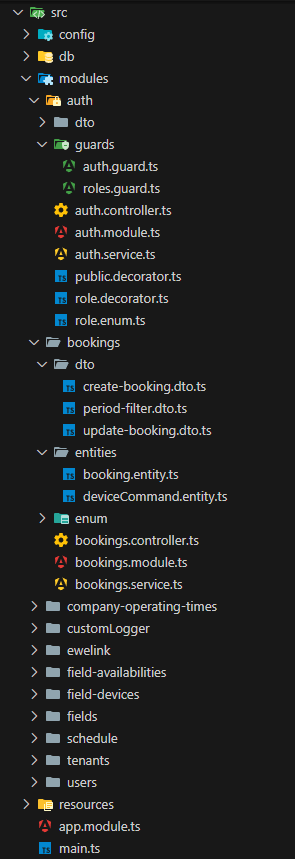
\includegraphics[scale=0.5]{images/cap5/arq_pastas.png}
	\end{center}
	\fonte{Autor.}
\end{figure}

\subsection{Implementação das Funcionalidades}\label{subsec:implementacao_funcionalidades}

Nessa seção serão detalhadas as implementações das funcionalidades do sistema. Serão abordados os modelos de dados \ref{subsubsec:modelagem_banco_dados}, autenticação e autorização \ref{subsubsec:autenticacao_autorizacao}, módulos de usuários \ref{subsubsec:modulo_usuarios}, tenants \ref{subsubsec:modulo_tenants}, quadras \ref{subsubsec:modulo_quadras}, disponibilidade de quadras \ref{subsubsec:modulo_disponibilidade_quadras}, integração com a API eWeLink \ref{subsubsec:integacao_ewelink}, quadras-dispositivos \ref{subsubsec:modulo_quadras_dispositivos}, reservas e comandos IoT \ref{subsubsec:modulo_reservas} e envio de comandos aos dispositivos IoT \ref{subsubsec:envio_comandos_iot}. Algumas rotas e implementações serão mostradas e detalhadas como exemplo e outras ocultadas a fim de reduzir a extensão do texto.

\subsubsection{Modelagem do Banco de Dados}\label{subsubsec:modelagem_banco_dados}
A primeira etapa do desenvolvimento do sistema é a modelagem do banco de dados. Nesta etapa, são criados os diagramas entidade-relacionamento (ER) que representam as entidades e seus relacionamentos. O diagrama ER é uma representação visual das tabelas do banco de dados e dos relacionamentos entre elas e está apresentado na \autoref{fig:modelagem_banco_dados}.

\begin{figure}[htp]
	\caption{\label{fig:modelagem_banco_dados}Modelagem do Banco de Dados.}
	\begin{center}
	  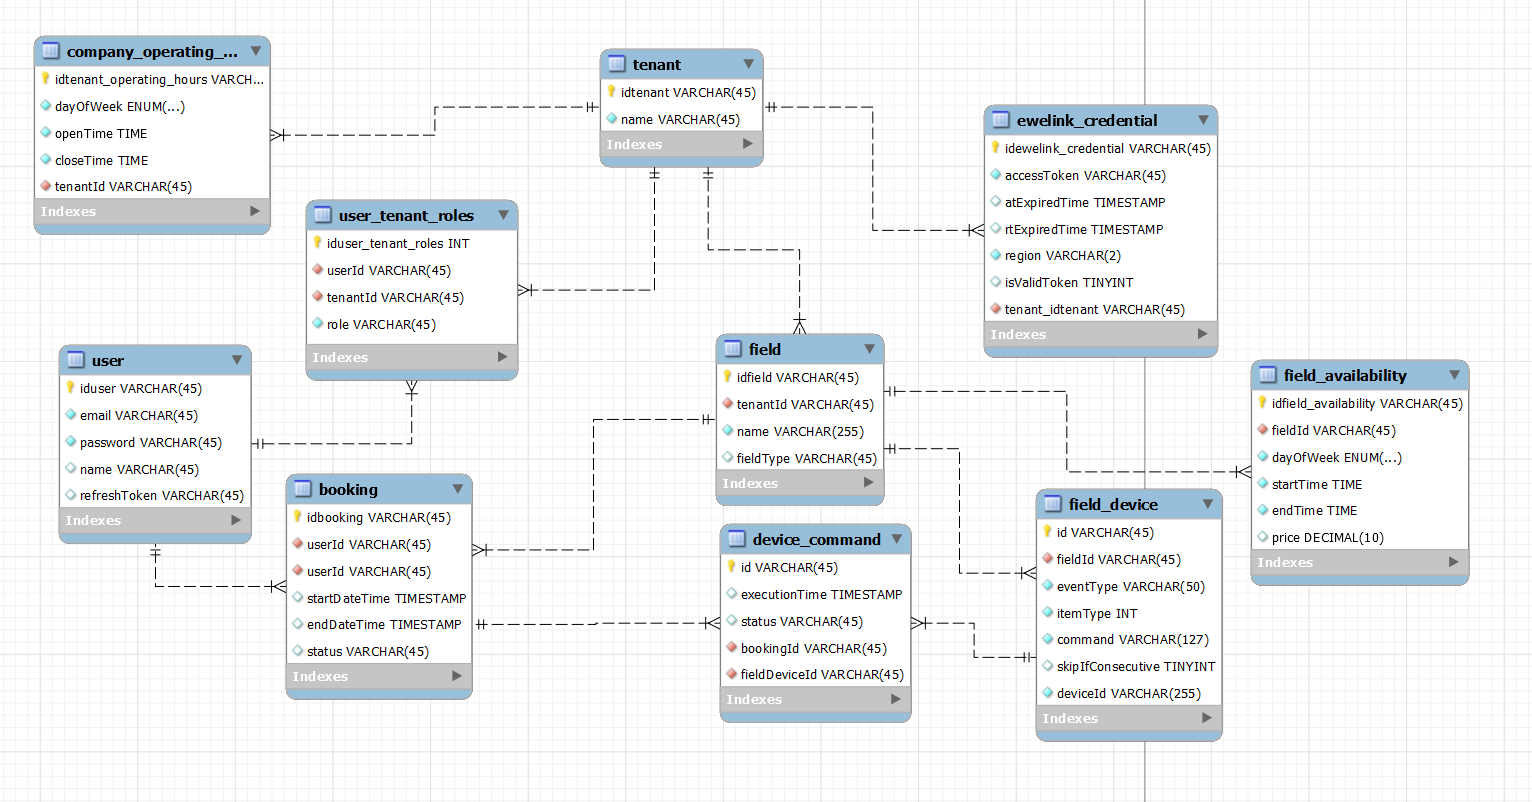
\includegraphics[scale=0.38]{images/cap5/modelage_banco_dados.png}
	\end{center}
	\fonte{Autor.}
\end{figure}

\textbf{tenant (Locatário/Empresa)}\\
Armazena informações das empresas que utilizam o sistema. Cada empresa tem um ambiente isolado para suas configurações e dados.\\
Relacionamentos:
\begin{itemize}
	\item Relaciona-se com \texttt{field} (uma empresa pode ter várias quadras).
	\item Relaciona-se com \texttt{user\_tenant\_roles} (definição de papéis dos usuários dentro da empresa).
	\item Relaciona-se com \texttt{ewelink\_credential} (armazenamento de credenciais IoT por empresa).
	\item Relaciona-se com \texttt{company\_operating\_hours} (definição do horário de funcionamento da empresa).
\end{itemize}

\textbf{user (Usuário do Sistema)}\\
Cadastra usuários na plataforma, permitindo o acesso e gestão de informações dos usuários em diferentes locatários. \\
Relacionamentos: 
\begin{itemize} 
	\item Relaciona-se com \texttt{use\_tenant\_roles} (um usuário pode ter diferentes papéis em empresas distintas). 
	\item Relaciona-se com \texttt{booking} (usuários realizam reservas de quadras). 
\end{itemize}

\textbf{user\textunderscore tenant\textunderscore roles (Papéis de Usuário na Empresa)}\\
Define os papéis dos usuários em diferentes locatários, garantindo acesso e permissões personalizadas para cada perfil. \\
Relacionamentos: 

\begin{itemize} 
	\item Relaciona-se com \texttt{user} (indica o usuário). 
	\item Relaciona-se com \texttt{tenant} (indica a empresa onde o usuário tem um papel). 
\end{itemize}


\textbf{company\textunderscore operating\textunderscore hours (Horários de Funcionamento da Empresa)}\\
Define os horários de funcionamento das empresas, permitindo customização e gestão do tempo disponível para operações em cada locatário. \\
Relacionamentos: 

\begin{itemize} 
	\item Relaciona-se com \texttt{tenant} (cada locatário tem seus próprios horários de funcionamento). 
\end{itemize}


\textbf{field (Quadras Esportivas)}\\
Armazena as quadras disponíveis para reservas, relacionadas ao locatário que as possui e contendo informações específicas sobre cada quadra. \\
Relacionamentos: 

\begin{itemize} 
	\item Relaciona-se com \texttt{tenant} (cada locatário pode ter várias quadras). 
	\item Relaciona-se com \texttt{field\_availability} (definição de horários disponíveis para a quadra). 
	\item Relaciona-se com \texttt{field\_device} (dispositivos IoT associados à quadra). 
	\item Relaciona-se com \texttt{booking} (quadras podem ser reservadas). 
\end{itemize}


\textbf{field\textunderscore availability (Disponibilidade da Quadra)}\\
Determina os horários disponíveis para cada quadra, indicando o período de tempo em que a mesma fica aberta e quanto custa o uso dela. \\
Relacionamentos: 

\begin{itemize} 
	\item Relaciona-se com \texttt{field} (define a disponibilidade para cada quadra). 
\end{itemize}


\textbf{booking (Reservas de Quadras)}\\
Registra as reservas feitas pelos usuários, associando-as ao locatário que possui a quadra reservada e outros detalhes sobre o horário, usuário e status da reserva. \\
Relacionamentos: 

\begin{itemize} 
	\item Relaciona-se com \texttt{user} (quem fez a reserva). 
	\item Relaciona-se com \texttt{field} (qual quadra foi reservada). 
\end{itemize}


\textbf{ewelink\textunderscore credential (Credenciais para Controle IoT via eWeLink)}\\
Armazena informações de autenticação da integração entre o sistema e dispositivos IoT, como tokens de acesso e gerenciamento de recursos. \\
Relacionamentos: 

\begin{itemize} 
	\item Relaciona-se com \texttt{tenant} (cada locatário pode ter credenciais IoT). 
\end{itemize}


\textbf{field\textunderscore device (Dispositivos IoT Associados às Quadras)}\\
Registra os dispositivos IoT instalados em cada quadra, indicando seu tipo de funcionalidade, comando a ser executado e outros detalhes relevantes para o gerenciamento. \\
Relacionamentos: 

\begin{itemize} 
	\item Relaciona-se com \texttt{field} (cada quadra pode ter vários dispositivos IoT). 
\end{itemize}


\textbf{device\textunderscore command (Comandos Enviados a Dispositivos IoT)}\\
Armazena os comandos programados ou executados para dispositivos IoT, associados às reservas e que devem ser executados conforme a agenda de reservas. \\
Relacionamentos: 

\begin{itemize} 
	\item Relaciona-se com \texttt{booking} (comandos são acionados conforme reservas). 
	\item Relaciona-se com \texttt{field\_device} (cada comando pertence a um dispositivo IoT). 
\end{itemize}

\subsubsection{Autenticação e Autorização}\label{subsubsec:autenticacao_autorizacao}

\textbf{Visão Geral}\\
O módulo de autenticação é responsável por garantir a segurança e o controle de acesso ao sistema multi-tenant. Ele permite que os usuários se autentiquem utilizando credenciais seguras e fornece mecanismos para gerenciamento de tokens de acesso e renovação de sessão. O sistema utiliza autenticação baseada em tokens JWT (\textit{JSON Web Token}) e cookies para armazenar \textit{refresh tokens} com segurança.

A autenticação dos usuários é fundamental para garantir que apenas indivíduos autorizados tenham acesso aos recursos do sistema. Além disso, o módulo gerencia o login, o registro de novos usuários (inicialmente sem vínculo com nenhum \textit{tenant}), a renovação de tokens e o logout seguro, invalidando tokens de sessão comprometidos.

\textbf{Fluxo das Rotas}\\
O controlador de autenticação (\texttt{auth.controller.ts}) define os endpoints responsáveis pelo login, registro de novos usuários, renovação de tokens e logout. Ele interage com o serviço de autenticação (\texttt{auth.service.ts}), que contém a lógica de geração e validação de tokens, verificação de credenciais e manipulação segura de sessões.

\subsubsubsection{Autenticação de Usuário}
\begin{itemize}
	\item \textbf{Rota:} \texttt{POST /auth/login}
	\item \textbf{Descrição:} Permite que um usuário se autentique utilizando seu e-mail e senha. Retorna um \textit{access token} e um \textit{refresh token}.
	\item \textbf{Fluxo:}
	\begin{enumerate}
		\item O controlador recebe as credenciais do usuário.
		\item O serviço de autenticação busca o usuário no banco de dados e valida a senha.
		\item Se as credenciais forem válidas, um novo \textit{access token} e um \textit{refresh token} são gerados e retornados.
	\end{enumerate}
\end{itemize}

O código construído para o \textit{controller} e  o \textit{service} estão disponíveis no \autoref{cod:login-controller} e  no \autoref{cod:login-service}, respectivamente, e servirão de exemplo para os demais \textit{controllers} e \textit{services}.

\begin{lstlisting}[caption={Exemplo de \textit{controller} para \textit{login}.},label={cod:login-controller}]
	@Post('login')
  async login(
    @Res({ passthrough: true }) res: Response,
    @Body() { email, password }: AuthenticateDto
  ) {
    const { loggedUser, accessToken, refreshToken } =
      await this.authService.login(email, password)

    res.cookie('jwt', refreshToken, {
      httpOnly: true,
      sameSite: 'none',
      secure: true,
      maxAge: 24 * 60 * 60 * 1000
    })
    res.status(201)
    return { accessToken, ...loggedUser }
  }
\end{lstlisting}

\begin{lstlisting}[caption={Exemplo de \textit{service} para \textit{login}.},label={cod:login-service}]
	async login(email: string, insertedPassword: string) {
    try {
      const foundUser = await this.userService.searchForEmail(email)

      const userWasAuthenticated = await bcrypt.compare(
        insertedPassword,
        foundUser.password
      )

      if (!userWasAuthenticated)
        throw new UnauthorizedException('E-mail e/ou senha incorretos.')

      const payload: UserPayload = {
        sub: foundUser.id,
        email: foundUser.email,
        name: foundUser.name
      }

      const newRefreshToken = await this.createRefreshToken(payload)
      const newAccessToken = await this.createAccessToken(payload)

      await this.updateRefreshToken(newRefreshToken, {
        sub: foundUser.id,
        ...foundUser
      })

      return {
        accessToken: newAccessToken,
        refreshToken: newRefreshToken,
        loggedUser: payload
      }
    } catch (e) {
      if (e?.status === 404 || e?.status === 401)
        throw new UnauthorizedException('E-mail e/ou senha incorretos.')

      console.log('Erro interno:', e)
      throw new InternalServerErrorException(
        'Erro interno no servidor. ' + e?.message
      )
    }
  }
\end{lstlisting}

\subsubsubsection{Registro de Usuário}
\begin{itemize}
	\item \textbf{Rota:} \texttt{POST /auth/register}
	\item \textbf{Descrição:} Permite criar um novo usuário no sistema sem vinculação com nenhuma empresa, armazenando suas credenciais de forma segura.
	\item \textbf{Fluxo:}
	\begin{enumerate}
		\item O controlador recebe os dados do novo usuário.
		\item A senha é criptografada antes de ser salva no banco de dados.
		\item O usuário é criado e retornado na resposta.
	\end{enumerate}
\end{itemize}

\subsubsubsection{Renovação de Token}
\begin{itemize}
	\item \textbf{Rota:} \texttt{GET /auth/refresh}
	\item \textbf{Descrição:} Permite gerar um novo \textit{access token} utilizando um \textit{refresh token} válido armazenado em um cookie.
	\item \textbf{Fluxo:}
	\begin{enumerate}
		\item O controlador verifica a presença do \textit{refresh token} nos cookies da requisição.
		\item O serviço valida o token e gera um novo \textit{access token}.
		\item O novo token é retornado na resposta.
	\end{enumerate}
\end{itemize}

\subsubsubsection{Logout}
\begin{itemize}
	\item \textbf{Rota:} \texttt{GET /auth/logout}
	\item \textbf{Descrição:} Invalida a sessão do usuário removendo seu \textit{refresh token} armazenado.
	\item \textbf{Fluxo:}
	\begin{enumerate}
		\item O controlador verifica o \textit{refresh token} armazenado no cookie da requisição.
		\item O serviço de autenticação invalida o token no banco de dados.
		\item O cookie é removido da resposta e a sessão é encerrada.
	\end{enumerate}
\end{itemize}

\subsubsection{Módulo de Tenants}\label{subsubsec:modulo_tenants}

\textbf{Visão Geral} \\
O módulo de \textit{tenants} é responsável por gerenciar múltiplos locatários dentro do sistema, permitindo a criação, consulta, atualização e remoção de \textit{tenants}. Esse módulo é essencial para suportar um ambiente multi-tenant, onde cada empresa ou cliente pode operar de forma isolada dentro da mesma aplicação.

As principais funcionalidades deste módulo incluem:

\begin{itemize}
    \item Criação de um \textit{tenant}, associando-o a um usuário administrador.
    \item Consulta de \textit{tenants}, tanto de forma individual quanto em lista.
    \item Atualização das informações de um \textit{tenant}.
    \item Remoção de um \textit{tenant}.
    \item Controle de permissões para diferentes níveis de usuário dentro de um \textit{tenant}.
\end{itemize}

O acesso às rotas do módulo é protegido por um sistema de autenticação e autorização baseado em \textit{roles}, garantindo que apenas usuários autorizados possam executar determinadas ações.

\textbf{Fluxo das Rotas} \\
As rotas do módulo de \textit{tenants} são definidas no \texttt{TenantsController}, garantindo a estruturação adequada dos endpoints da API. A seguir, estão dispostos os fluxos de duas das principais operações: criação e busca de \textit{tenants}.

\subsubsubsection{Criação de um Tenant}
\begin{itemize}
	\item \textbf{Rota:} \texttt{POST /tenants}
	\item \textbf{Descrição:} Criação de um novo \textit{tenant}.
	\item \textbf{Fluxo:}
	\begin{enumerate}
    \item O usuário autenticado envia uma requisição contendo os dados do novo \textit{tenant}.
    \item O serviço verifica se o usuário tem permissão para criar um \textit{tenant}.
    \item Se autorizado, os dados do \textit{tenant} são persistidos no banco de dados.
    \item O usuário criador recebe automaticamente o papel de administrador dentro do novo \textit{tenant}.
    \item A resposta retorna uma mensagem de sucesso e os detalhes do \textit{tenant} criado.
	\end{enumerate}
\end{itemize}

\subsubsubsection{Consulta de um Tenant}
\begin{itemize}
	\item \textbf{Rota:} \texttt{GET /tenants/:id}
	\item \textbf{Descrição:} Buscar um \textit{tenant} específico.
	\item \textbf{Fluxo:}
	\begin{enumerate}
    \item O usuário faz uma requisição com o identificador do \textit{tenant} desejado.
    \item O serviço consulta o banco de dados para localizar o \textit{tenant} correspondente.
    \item Se encontrado, os detalhes do \textit{tenant} são retornados na resposta.
    \item Se o \textit{tenant} não for encontrado, uma exceção é lançada informando o erro.
	\end{enumerate}
\end{itemize}

\textbf{Outras Operações} \\
Além das rotas descritas acima, o módulo também disponibiliza endpoints para listar todos os \textit{tenants}, atualizar informações e remover um \textit{tenant}. Estas operações são protegidas por um sistema de autenticação e autorização baseado em \textit{roles}, garantindo que apenas usuários com as permissões adequadas possam realizá-las.

\subsubsection{Módulo de Usuarios}\label{subsubsec:modulo_usuarios}

\textbf{Visão Geral}\\
O módulo de usuários é responsável por gerenciar os perfis de usuários dentro do sistema multi-tenant. Ele permite o cadastro, consulta, edição e remoção de usuários (vinculados a uma empresa específica), além de possibilitar a gestão de papéis dentro de diferentes empresas. O sistema suporta diferentes níveis de acesso e autenticação baseada em tokens.

Os usuários podem pertencer a múltiplas empresas e ter diferentes papéis em cada uma delas. Isso permite um controle granular das permissões e acesso às funcionalidades do sistema.

\textbf{Fluxo das Rotas}\\
O controlador de usuários (\texttt{users.controller.ts}) define os endpoints para interação com o serviço de usuários (\texttt{users.service.ts}), que contém a lógica de negócio. O código construído para o \textit{controller} e  o \textit{service} estão disponíveis no \autoref{cod:create-user-controller} e  no \autoref{cod:create-user-service}, respectivamente, e servirão de exemplo para os demais \textit{controllers} e \textit{services}.

\subsubsubsection{Criação de Usuário}
\begin{itemize}
	\item \textbf{Rota:} \texttt{POST /tenant/:tenantId/users}
	\item \textbf{Descrição:} Permite criar um novo usuário, recebendo os dados básicos no corpo da requisição. Caso seja informado um \texttt{tenantId}, o usuário é vinculado a essa empresa.
	\item \textbf{Fluxo:}
	\begin{enumerate}
		\item O controlador recebe os dados do novo usuário.
		\item O serviço cria a entidade e a salva no banco.
		\item O usuário é retornado na resposta.
	\end{enumerate}
\end{itemize}

\begin{lstlisting}[caption={Exemplo de \textit{controller} para criação de usuário.},label={cod:create-user-controller}]
	@Post()
  async createUser(
    @Body() { password, ...userData }: CreateUserDTO,
    @Body('password', HashingPasswordPipe) hashedPassword: string
  ) {
    const createdUser = await this.userService.createUser({
      ...userData,
      password: hashedPassword
    })

    return {
      message: 'Usuario criado!',
      user: new ListUserDTO({ id: createdUser.id, name: createdUser.name })
    }
  }
\end{lstlisting}

\begin{lstlisting}[caption={Exemplo de \textit{service} para criação de usuário.},label={cod:create-user-service}]
	async createUser(userData: CreateUserDTO, tenantId?: string) {
    const userEntity = new User()

    Object.assign(userEntity, userData as User)
    const createdUser = await this.userRepository.save(userEntity)

    console.log('Create relation to tenant: ', tenantId)

    return createdUser
  }
\end{lstlisting}

\subsubsubsection{Consulta de Usuário por ID}
\begin{itemize}
	\item \textbf{Rota:} \texttt{GET /tenant/:tenantId/users/:id}
	\item \textbf{Descrição:} Retorna as informações detalhadas de um usuário, incluindo seus papéis nas empresas.
	\item \textbf{Fluxo:}
	\begin{enumerate}
		\item O controlador recebe o \texttt{id} do usuário via parâmetro de rota.
		\item O serviço busca o usuário no banco, carregando as relações necessárias.
		\item Caso não seja encontrado, retorna erro.
		\item Se encontrado, retorna os dados do usuário.
	\end{enumerate}
\end{itemize}

\subsubsubsection{Listagem de Usuários de uma Empresa}
\begin{itemize}
	\item \textbf{Rota:} \texttt{GET /tenant/:tenantId/users}
	\item \textbf{Descrição:} Retorna uma lista de usuários vinculados a uma empresa.
	\item \textbf{Fluxo:}
	\begin{enumerate}
		\item O controlador recebe o \texttt{tenantId} como um parâmetro.
		\item O serviço busca os usuários que possuem relação com essa empresa.
		\item Retorna a lista formatada.
	\end{enumerate}
\end{itemize}

\subsubsubsection{Atualização de Usuário}
\begin{itemize}
  \item \textbf{Rota:} \texttt{PATCH /tenant/:tenantId/users/:id}
  \item \textbf{Descrição:} Permite a edição dos dados cadastrais de um usuário.
  \item \textbf{Fluxo:}
  \begin{enumerate}
    \item O controlador recebe o \texttt{id} e os novos dados do usuário.
    \item O serviço verifica se o usuário existe.
    \item Caso não exista, retorna erro.
    \item Atualiza os dados e os salva no banco.
    \item Retorna os novos dados do usuário.
  \end{enumerate}
\end{itemize}

\subsubsubsection{Atualização de Papel de Usuário}
\begin{itemize}
  \item \textbf{Rota:} \texttt{PATCH /tenant/:tenantId/users/:id/role}
  \item \textbf{Descrição:} Atualiza o papel do usuário dentro de uma empresa.
  \item \textbf{Fluxo:}
  \begin{enumerate}
    \item O controlador recebe o \texttt{id} do usuário, o \texttt{tenantId} e o novo papel.
    \item O serviço verifica se o papel existe.
    \item O serviço verifica se o usuário solicitante tem permissão para a alteração.
    \item Caso não tenha permissão, retorna erro.
    \item Atualiza o papel e salva no banco.
    \item Retorna os novos dados do usuário.
  \end{enumerate}
\end{itemize}

\subsubsubsection{Exclusão de Usuário}
\begin{itemize}
  \item \textbf{Rota:} \texttt{DELETE /tenant/:tenantId/users/:id}
  \item \textbf{Descrição:} Remove um usuário do sistema (exclusão lógica).
  \item \textbf{Fluxo:}
  \begin{enumerate}
    \item O controlador recebe o \texttt{id} do usuário.
    \item O serviço verifica se o usuário existe.
    \item Caso não exista, retorna erro.
    \item Apaga logicamente o registro do banco.
    \item Retorna sucesso.
  \end{enumerate}
\end{itemize}

\textbf{Conclusão} \\
Esse módulo é essencial para a gestão dos usuários do sistema, garantindo que cada um tenha acesso adequado aos recursos da empresa em que está vinculado. As regras de permissão asseguram que apenas usuários autorizados possam modificar informações sensíveis, proporcionando segurança e integridade aos dados.

\subsubsection{Módulos de Quadras e Disponibilidade de Quadras}\label{subsubsec:modulos_quadras_disponibilidade_quadras}

\textbf{Visão Geral}\\
Os módulos de \textit{quadras} e \textit{disponibilidade de quadras} são responsáveis pelo gerenciamento dos espaços esportivos disponíveis para reserva dentro do sistema. O módulo de quadras gerencia a criação, consulta, atualização e remoção das quadras cadastradas, enquanto o módulo de disponibilidade de quadras permite definir os horários disponíveis para cada quadra em dias específicos da semana.

As principais funcionalidades destes módulos incluem:

\begin{itemize}
    \item Criação e gerenciamento das quadras dentro de um \textit{tenant}.
    \item Definição de horários disponíveis para cada quadra.
    \item Consulta das quadras e suas disponibilidades.
    \item Atualização e remoção de quadras e horários disponíveis.
\end{itemize}

\textbf{Fluxo das Rotas}\\
As rotas desses módulos são definidas nos controladores \texttt{FieldsController} e \texttt{FieldAvailabilitiesController}. A seguir, estão dispostos os fluxos das operações de criação e consulta de quadras e disponibilidade.

\subsubsubsection{Criação de uma Quadra}
\begin{itemize}
    \item \textbf{Rota:} \texttt{POST /tenants/:tenantId/fields}
    \item \textbf{Descrição:} Criar uma nova quadra dentro de um \textit{tenant}.
    \item \textbf{Fluxo:}
    \begin{enumerate}
        \item O usuário autenticado com permissão faz uma requisição contendo os dados da nova quadra.
        \item O serviço verifica se o \textit{tenant} informado existe.
        \item Se autorizado, os dados da quadra são persistidos no banco de dados.
        \item A resposta retorna uma mensagem de sucesso e os detalhes da quadra criada.
    \end{enumerate}
\end{itemize}

\subsubsubsection{Consulta de uma Quadra}
\begin{itemize}
    \item \textbf{Rota:} \texttt{GET /tenants/:tenantId/fields/:id}
    \item \textbf{Descrição:} Buscar uma quadra específica dentro de um \textit{tenant}.
    \item \textbf{Fluxo:}
    \begin{enumerate}
        \item O usuário faz uma requisição com o identificador da quadra e do \textit{tenant}.
        \item O serviço consulta o banco de dados para localizar a quadra correspondente.
        \item Se encontrada, os detalhes da quadra são retornados na resposta.
        \item Se a quadra não for encontrada, uma exceção é lançada informando o erro.
    \end{enumerate}
\end{itemize}

\subsubsubsection{Criação de Disponibilidade de Quadra}
\begin{itemize}
    \item \textbf{Rota:} \texttt{POST /tenants/:tenantId/fields/:fieldId/field-availabilities}
    \item \textbf{Descrição:} Criar um ou mais horários disponíveis para uma quadra específica.
    \item \textbf{Fluxo:}
    \begin{enumerate}
        \item O usuário autenticado com permissão faz uma requisição contendo os horários disponíveis para uma quadra.
        \item O serviço verifica se a quadra informada existe.
        \item Se validado, os horários são armazenados no banco de dados.
        \item A resposta retorna a confirmação da criação dos horários.
    \end{enumerate}
\end{itemize}

\subsubsubsection{Consulta de Disponibilidade de Quadra}
\begin{itemize}
    \item \textbf{Rota:} \texttt{GET /tenants/:tenantId/fields/:fieldId/field-availabilities/:id}
    \item \textbf{Descrição:} Buscar um horário de disponibilidade específico de uma quadra.
    \item \textbf{Fluxo:}
    \begin{enumerate}
        \item O usuário faz uma requisição com o identificador da disponibilidade e da quadra correspondente.
        \item O serviço consulta o banco de dados para localizar o horário correspondente.
        \item Se encontrado, os detalhes da disponibilidade são retornados na resposta.
        \item Se o horário não for encontrado, uma exceção é lançada informando o erro.
    \end{enumerate}
\end{itemize}

\textbf{Outras Operações}\\
Além das rotas descritas acima, os módulos também disponibilizam endpoints para listar todas as quadras, atualizar informações e remover quadras e horários disponíveis.

\subsubsection{Integração com eWeLink}\label{subsubsec:integacao_ewelink}

\textbf{Visão Geral} \\
O módulo de integração com a API eWeLink é responsável por permitir a conexão entre o sistema e dispositivos IoT suportados pela plataforma eWeLink. Ele possibilita que os administradores das empresas associem sua conta à plataforma, consultem os seus dispositivos e interajam de forma automatizada com os equipamentos cadastrados.

As principais funcionalidades deste módulo incluem:

\begin{itemize}
    \item Autenticação de usuários na API eWeLink via OAuth2.0 para permitir o gerenciamento dos dispositivos pela plataforma.
    \item Consulta e listagem dos dispositivos vinculados a um determinado \textit{tenant}.
    \item Atualização e renovação automática dos tokens de acesso à API eWeLink.
    \item Controle seguro de permissões, garantindo que apenas administradores possam gerenciar dispositivos.
\end{itemize}

\textbf{Fluxo das Rotas} \\
As rotas deste módulo são definidas no \texttt{EwelinkController} e interagem com o serviço de autenticação e gerenciamento de dispositivos eWeLink, fornecido pelo \texttt{EwelinkService}. A seguir, apresenta-se o fluxo das operações deste módulo.

\subsubsubsection{Autenticação na API eWeLink}
\begin{itemize}
    \item \textbf{Rota:} \texttt{GET /tenants/:tenantId/ewelink/login}
    \item \textbf{Descrição:} Redireciona o usuário para a página de autenticação da eWeLink.
    \item \textbf{Fluxo:}
    \begin{enumerate}
        \item O usuário autenticado faz uma requisição para iniciar a autenticação com a API eWeLink.
        \item O serviço gera uma URL de autenticação com a informação do \texttt{tenantId} e redireciona o usuário para a página de login da eWeLink.
        \item Após a autenticação bem-sucedida, a eWeLink redireciona o usuário de volta ao sistema com um código de autorização através do \texttt{tenantId}.
    \end{enumerate}
\end{itemize}

Esse fluxo de autenticação segue o formato OAuth2.0. OAuth (Open Authorization) 2.0 é um protocolo padrão para autorização de acesso a recursos online. Ele permite que um cliente solicite permissão específica do usuário para o acesso a dados ou serviços, sem compartilhar informações sensitivas diretamente com o provedor de recursos. OAuth2.0 define quatro protocolos:

\begin{enumerate}
  \item Autorização de Cliente (Client Authorization): o cliente solicita permissão ao usuário para autorizar o acesso à aplicação web ou dispositivo móvel que deseja usar os recursos do provedor de recursos.
  \item Tokens de Acesso (Access Tokens): o provedor de recursos concede um token de acesso ao cliente, que é utilizado para autenticar futuras solicitações e obter acesso aos recursos protegidos.
  \item Refresh Tokens: quando o token de acesso expira ou está prestes a fazer isso, o cliente pode usar o refresh token para obter um novo token sem reautenticar o usuário.
  \item Gerenciamento de Autorização (Authorization Management): o provedor de recursos permite que os administradores revoguem ou gerenciem as permissões concedidas a um cliente.
\end{enumerate}

O fluxo geral do protocolo OAuth2.0 é o seguinte:

\begin{enumerate}
  \item Autenticação do Usuário: o usuário realiza autenticação no provedor de recursos.
  \item Solicitando Autorização: a aplicação web ou dispositivo móvel solicita permissão ao usuário para acessar um recurso protegido em nome do usuário.
  \item Autorização de Cliente: o provedor de recursos exibe uma janela à qual o cliente pode dar autorização à aplicação web ou dispositivo móvel.
  \item Gerando Tokens de Acesso e Refresh Tokens: se o usuário concede a autorização, o provedor de recursos gera um token de acesso e um refresh token (se for o caso).
  \item Recebendo e Utilizando Tokens de Acesso: a aplicação web ou dispositivo móvel envia o token de acesso para solicitar os recursos protegidos.
  \item Verificando e Renovando Tokens de Acesso: quando o token de acesso expira, a aplicação web ou dispositivo móvel usa o refresh token para obter um novo token sem reautenticar o usuário.
\end{enumerate}

OAuth2.0 é amplamente utilizado em plataformas online, como Google Drive, Facebook e Twitter, que promove a autorização segura de recursos entre diferentes aplicações.

\begin{figure}[htp]
	\caption{\label{fig:oauth1}OAuth2.0 EWeLink. Obter oauth \textit{token}}
	\begin{center}
	  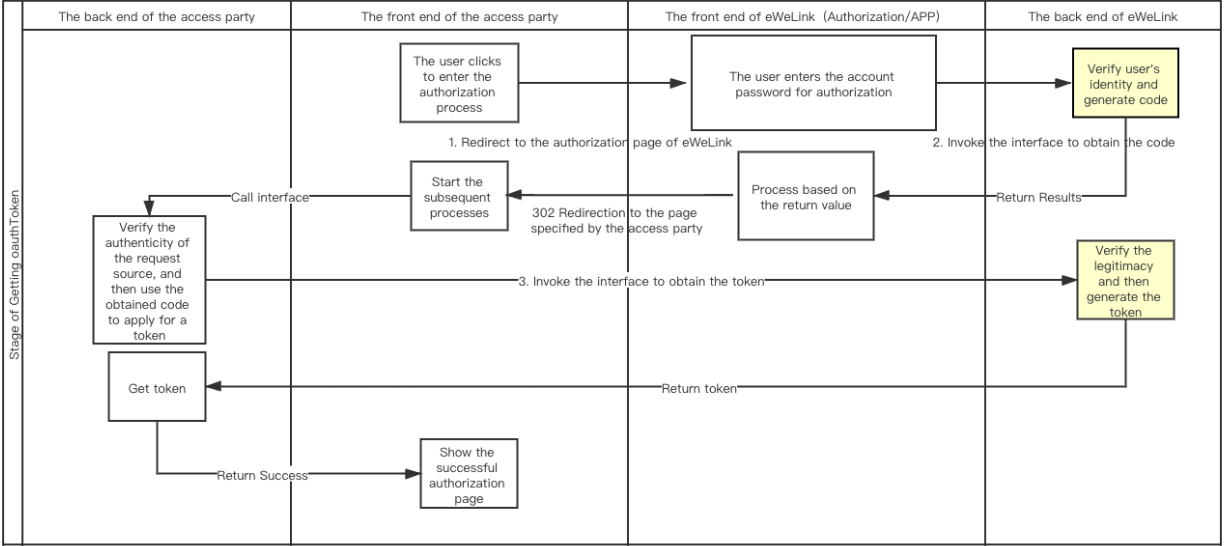
\includegraphics[scale=0.45]{images/cap5/oauth_1.png}
	\end{center}
	\fonte{\cite{COOLKITOAUTH}}
\end{figure}

No contexto da aplicação desenvolvida neste PFC, o usuário é redirecionado para a página de autenticação da eWeLink, onde ele pode inserir suas credenciais. Após o login bem-sucedido, a eWeLink redireciona o usuário de volta ao sistema com um código de autorização (\textit{access token}) conforme demonstrado na \autoref{fig:oauth1}, que é armazenado no banco de dados para permitir interações futuras com a API.

\subsubsubsection{Obtenção do Token de Acesso eWeLink}
\begin{itemize}
    \item \textbf{Rota:} \texttt{GET /ewelink/redirectUrl}
    \item \textbf{Descrição:} Recebe o código de autorização da eWeLink e gera um token de acesso.
    \item \textbf{Fluxo:}
    \begin{enumerate}
        \item O usuário é redirecionado da eWeLink para o sistema com um código de autorização.
        \item O sistema utiliza esse código para obter um token de acesso e um token de atualização.
        \item As credenciais são armazenadas no banco de dados para permitir interações futuras com a API.
    \end{enumerate}
\end{itemize}

\subsubsubsection{Listagem de Dispositivos eWeLink}
\begin{itemize}
    \item \textbf{Rota:} \texttt{POST /tenants/:tenantId/ewelink/listAllThings}
    \item \textbf{Descrição:} Lista todos os dispositivos associados a um determinado \textit{tenant}.
    \item \textbf{Fluxo:}
    \begin{enumerate}
        \item O usuário autenticado com permissão faz uma requisição para listar os dispositivos.
        \item O serviço verifica as credenciais e atualiza os tokens se necessário.
        \item O serviço consulta a API eWeLink e retorna a lista de dispositivos cadastrados.
    \end{enumerate}
\end{itemize}

\begin{figure}[htp]
	\caption{\label{fig:oauth2}OAuth2.0 EWeLink. Usando um \textit{access token}}
	\begin{center}
	  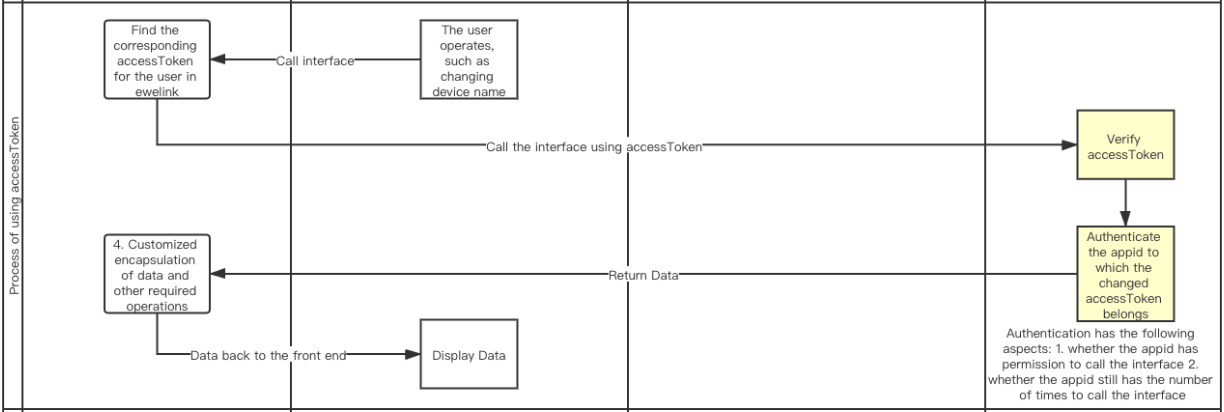
\includegraphics[scale=0.45]{images/cap5/oauth_2.png}
	\end{center}
	\fonte{\cite{COOLKITOAUTH}}
\end{figure}

A \autoref{fig:oauth2} mostra o processo de uso do \textit{access token} na interação com a plataforma \textit{Coolkit Open Platform 4.3 EWeLink}. Neste exemplo, o usuário autenticado com permissão realiza uma requisição para listar os dispositivos, que são consultados na API eWeLink e retornados ao usuário.

\begin{figure}[htp]
	\caption{\label{fig:oauth3}OAuth2.0 EWeLink. Atualizando um \textit{access token}}
	\begin{center}
	  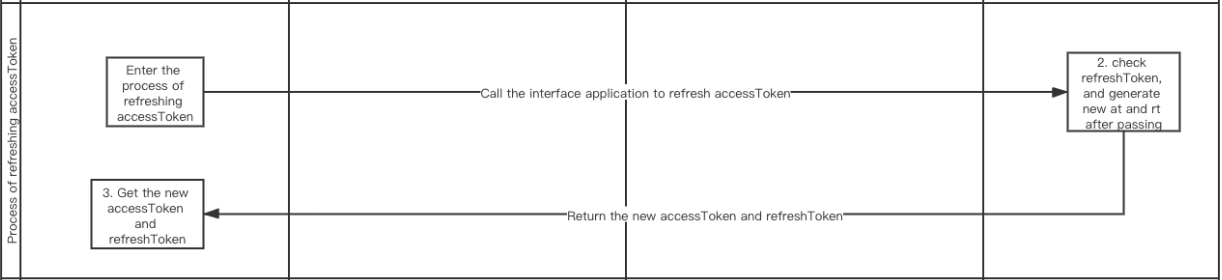
\includegraphics[scale=0.45]{images/cap5/oauth_3.png}
	\end{center}
	\fonte{\cite{COOLKITOAUTH}}
\end{figure}

Caso o \textit{access token} esteja expirado ou inválido, a aplicação solicita um novo token utilizando o \textit{refresh token}. O servidor de autorização gera um novo \textit{access token} e um novo \textit{refresh token}, que podem ser usados para futuras requisições. Caso o \textit{refresh token} esteja expirado ou inválido, a plataforma acusará erro e indicará ao usuário para efetuar login novamente para obter um novo \textit{access token} e \textit{refresh token}.
 
\textbf{Outras Operações}\\
Além das rotas descritas acima, o módulo também inclui funcionalidades para atualização de tokens de acesso, controle de status dos dispositivos e integração com eventos IoT.

\subsubsection{Módulo de Quadras-Dispositivos}\label{subsubsec:modulo_quadras_dispositivos}

\textbf{Visão Geral}\\
O módulo de \textit{field-devices} é responsável pela integração entre as quadras esportivas e os dispositivos IoT, permitindo o gerenciamento dos equipamentos eletrônicos associados a cada quadra. Essa funcionalidade possibilita o controle automatizado de iluminação, climatização e outros dispositivos conectados, otimizando a experiência do usuário e a gestão operacional do sistema.

As principais funcionalidades deste módulo incluem:

\begin{itemize}
\item Associação de comandos de dispositivos a quadras esportivas específicas.
\item Consulta e listagem dos comandos de dispositivos cadastrados para uma quadra.
\item Atualização e remoção de dispositivos vinculados às quadras.
\item Controle seguro de permissões, garantindo que apenas administradores e gerentes possam gerenciar os dispositivos.
\end{itemize}

\textbf{Fluxo das Rotas}\\
As rotas deste módulo são definidas no \texttt{FieldDevicesController} e interagem com o serviço de gerenciamento de dispositivos \texttt{FieldDevicesService}. A seguir, são apresentados os fluxos de todas as operações disponíveis.

\subsubsubsection{Criação de um Dispositivo de Quadra}
\begin{itemize}
\item \textbf{Rota:} \texttt{POST /tenants/:tenantId/fields/:fieldId/field-devices}
\item \textbf{Descrição:} Criar um novo comando de dispositivo vinculado a uma quadra esportiva.
\item \textbf{Fluxo:}
\begin{enumerate}
\item O usuário autenticado com permissão faz uma requisição contendo os dados do dispositivo obtidos através da API eWeLink juntamente com o comando desejado.
\item O serviço verifica se a quadra informada existe.
\item Se validado, os dados do dispositivo e o comando desejado são armazenados no banco de dados e associados à quadra.
\item A resposta retorna uma mensagem de sucesso e os detalhes do dispositivo cadastrado.
\end{enumerate}
\end{itemize}

\subsubsubsection{Consulta de Todos os Dispositivos de uma Quadra}
\begin{itemize}
\item \textbf{Rota:} \texttt{GET /tenants/:tenantId/fields/:fieldId/field-devices}
\item \textbf{Descrição:} Retorna uma lista com todos os dispositivos vinculados a uma quadra específica.
\item \textbf{Fluxo:}
\begin{enumerate}
\item O usuário faz uma requisição para listar os dispositivos de uma quadra específica.
\item O serviço busca todos os dispositivos associados à quadra no banco de dados.
\item A lista dos dispositivos cadastrados é retornada na resposta.
\end{enumerate}
\end{itemize}

\subsubsubsection{Consulta de um Dispositivo de Quadra Específico}
\begin{itemize}
\item \textbf{Rota:} \texttt{GET /tenants/:tenantId/fields/:fieldId/field-devices/:id}
\item \textbf{Descrição:} Buscar um dispositivo específico vinculado a uma quadra esportiva.
\item \textbf{Fluxo:}
\begin{enumerate}
\item O usuário faz uma requisição com o identificador do dispositivo e da quadra correspondente.
\item O serviço consulta o banco de dados para localizar o dispositivo correspondente.
\item Se encontrado, os detalhes do dispositivo são retornados na resposta.
\item Se o dispositivo não for encontrado, uma exceção é lançada informando o erro.
\end{enumerate}
\end{itemize}

\subsubsubsection{Atualização de um Dispositivo de Quadra}
\begin{itemize}
\item \textbf{Rota:} \texttt{PATCH /tenants/:tenantId/fields/:fieldId/field-devices/:id}
\item \textbf{Descrição:} Atualiza as informações de um comando de dispositivo vinculado a uma quadra esportiva.
\item \textbf{Fluxo:}
\begin{enumerate}
\item O usuário autenticado com permissão faz uma requisição contendo os dados atualizados do dispositivo.
\item O serviço verifica se o dispositivo informado existe.
\item Se validado, os dados do dispositivo são atualizados no banco de dados.
\item A resposta retorna uma mensagem de sucesso e os detalhes do dispositivo atualizado.
\end{enumerate}
\end{itemize}

\subsubsubsection{Remoção de um Dispositivo de Quadra}
\begin{itemize}
\item \textbf{Rota:} \texttt{DELETE /tenants/:tenantId/fields/:fieldId/field-devices/:id}
\item \textbf{Descrição:} Remove um comando de dispositivo vinculado a uma quadra esportiva.
\item \textbf{Fluxo:}
\begin{enumerate}
\item O usuário autenticado com permissão faz uma requisição para remover o dispositivo.
\item O serviço verifica se o dispositivo informado existe.
\item Se encontrado, o dispositivo é removido logicamente do banco de dados.
\item A resposta confirma a remoção do dispositivo.
\end{enumerate}
\end{itemize}

\subsubsection{Módulo de Reservas e Comandos IoT}\label{subsubsec:modulo_reservas}

\textbf{Visão Geral}\\
O módulo de \textit{reservas e comandos IoT} é responsável pelo gerenciamento das reservas de quadras esportivas e pela automação dos dispositivos IoT associados. Ele garante que os usuários possam realizar reservas de maneira eficiente, ao mesmo tempo que controla dispositivos como iluminação e climatização, otimizando os recursos disponíveis.

As principais funcionalidades deste módulo incluem:

\begin{itemize}
    \item Criação e gerenciamento de reservas de quadras esportivas.
    \item Listagem de reservas existentes, incluindo filtros por período e usuário.
    \item Controle automatizado de dispositivos IoT com base nos horários das reservas.
    \item Prevenção de conflitos de horários e gerenciamento de comandos consecutivos para dispositivos.
\end{itemize}

\textbf{Fluxo das Rotas}\\
As rotas deste módulo são definidas no \texttt{BookingsController} e interagem com o serviço de gerenciamento de reservas e automação de dispositivos IoT, fornecido pelo \texttt{BookingsService}. A seguir, são apresentados os fluxos das principais operações disponíveis.

\subsubsubsection{Criação de uma Reserva}
\begin{itemize}
    \item \textbf{Rota:} \texttt{POST /tenants/:tenantId/fields/:fieldId/bookings}
    \item \textbf{Descrição:} Criar uma nova reserva para uma quadra esportiva.
    \item \textbf{Fluxo:}
    \begin{enumerate}
        \item O usuário autenticado com permissão faz uma requisição contendo os detalhes da reserva.
        \item O serviço verifica se a quadra informada existe e se a disponibilidade está correta.
        \item Caso não haja conflitos de horário, a reserva é criada e armazenada no banco de dados.
        \item Se houver dispositivos IoT associados à quadra, são criados comandos automáticos para acioná-los no início e no final da reserva.
        \item A resposta retorna uma mensagem de sucesso com os detalhes da reserva e dos comandos IoT gerados.
    \end{enumerate}
\end{itemize}

O código construído para o o \textit{service} está disponíveis no \autoref{cod:create-booking-service}.

\begin{lstlisting}[caption={Exemplo de \textit{controller} para \textit{login}.},label={cod:create-booking-service}]
	async create(
    createBookingDto: CreateBookingDto,
    fieldId: string,
    userId: string
  ) {
    const fieldAvailability = await this.fieldAvailabilitiesService.findOne(
      fieldId,
      createBookingDto.fieldAvailabilityId
    )

    const user = await this.usersService.findById(userId)

    const startDateTime = moment(createBookingDto.startTime)
    const endDateTime = moment(createBookingDto.endTime)
    console.log('startDateTime moment', startDateTime)
    console.log('endDateTime moment', endDateTime)

    const hasConflict = await this.hasBookingConflict(
      fieldId,
      createBookingDto.startTime,
      createBookingDto.endTime
    )

    if (hasConflict)
      throw new ConflictException('Ja existe uma reserva neste periodo')

    // check if the week days are the same
    if (
      startDateTime.utc().day() !==
      moment().day(fieldAvailability.dayOfWeek).day()
    )
      throw new BadRequestException(
        'Dia da semana solicitado nao confere com o dia disponivel'
      )

    // check if the start and end times match the availability range
    if (
      startDateTime.utc().format('HH:mm:ss') !== fieldAvailability.startTime ||
      endDateTime.utc().format('HH:mm:ss') !== fieldAvailability.endTime
    ) {
      console.log('hora disponivel inicio:', fieldAvailability.startTime)
      console.log(
        'hora solicitada inicio:',
        startDateTime.utc().format('HH:mm:ss')
      )
      console.log('hora disponivel final:', fieldAvailability.endTime)
      console.log(
        'hora solicitada final:',
        endDateTime.utc().format('HH:mm:ss')
      )

      throw new BadRequestException(
        'Horarios solicitados nao conferem com os horarios disponiveis'
      )
    }

    const booking = new Booking()

    Object.assign(booking, {
      ...createBookingDto,
      field: fieldAvailability.field,
      user
    } as unknown as Booking)
    // Filter data to return without user for the booking
    const createdBooking = await this.bookingsRepository.save(booking)

    const fieldDevicesByField = await this.fieldDevicesService.findAll(fieldId)

    // if there are field devices, create device commands
    const returnObject = { booking: createdBooking }
    if (fieldDevicesByField.length > 0) {
      const bookingDeviceCommands = fieldDevicesByField.map((device) => {
        const deviceCommand = new DeviceCommand()
        Object.assign(deviceCommand, {
          booking: createdBooking,
          fieldDevice: device,
          executionTime:
            device.eventType === EventTypeEnum.START
              ? booking.startTime
              : booking.endTime
        })
        return deviceCommand
      })

      const consecutiveCommands = await Promise.all(
        bookingDeviceCommands.map((command) => {
          // Step 1: Check if there are any consecutive commands for the same device and ignore them
          const query = {
            where: {
              status: CommandStatusEnum.PENDING,
              fieldDevice: {
                deviceId: command.fieldDevice.deviceId,
                skipIfConsecutive: true,
                field: { id: fieldId }
              },
              executionTime: Between(
                moment(command.executionTime).subtract(5, 'minutes').toDate(),
                moment(command.executionTime).add(5, 'minutes').toDate()
              )
            },
            relations: { fieldDevice: { field: true } }
          }
          return this.deviceCommandsRepository.findOne(query)
        })
      )

      // search if the command has any consecutive command so it needs to be ignored
      const deviceCommandsWithoutConsecutiveCommands =
        bookingDeviceCommands.filter(
          (_command, index) => !consecutiveCommands[index]
        )

      // delete the pending commands that are already in the device_command table
      const commandsToDeleteFromDeviceCommandTable = consecutiveCommands.filter(
        (command) => !!command
      )

      // delete the commands from the device_command table
      if (commandsToDeleteFromDeviceCommandTable.length > 0) {
        await this.deviceCommandsRepository.delete(
          commandsToDeleteFromDeviceCommandTable.map((command) => command.id)
        )

        returnObject['deviceCommandsDeleted'] =
          commandsToDeleteFromDeviceCommandTable
      }
      returnObject['deviceCommandsCreated'] =
        await this.deviceCommandsRepository.save(
          deviceCommandsWithoutConsecutiveCommands
        )
    }

    return returnObject
  }

  async hasBookingConflict(
    fieldId: string,
    startTime: string,
    endTime: string
  ): Promise<boolean> {
    const conflict = await this.bookingsRepository.query(
      `SELECT COUNT(*) > 0 AS has_overlap
      FROM booking
      WHERE "fieldId" = $1
        AND "startTime" < $3
        AND "endTime" > $2`,
      [fieldId, startTime, endTime]
    )
    return conflict[0]?.has_overlap
  }
\end{lstlisting}

\subsubsubsection{Listagem de Reservas de uma Quadra}
\begin{itemize}
    \item \textbf{Rota:} \texttt{GET /tenants/:tenantId/fields/:fieldId/bookings}
    \item \textbf{Descrição:} Retorna todas as reservas vinculadas a uma quadra específica.
    \item \textbf{Fluxo:}
    \begin{enumerate}
        \item O usuário faz uma requisição para listar as reservas de uma quadra específica.
        \item O serviço busca todas as reservas associadas à quadra no banco de dados.
        \item A lista das reservas cadastradas é retornada na resposta.
    \end{enumerate}
\end{itemize}

\subsubsubsection{Listagem de Reservas Futuras por Período}
\begin{itemize}
    \item \textbf{Rota:} \texttt{POST /tenants/:tenantId/fields/:fieldId/bookings/future}
    \item \textbf{Descrição:} Retorna todas as reservas futuras dentro de um determinado período.
    \item \textbf{Fluxo:}
    \begin{enumerate}
        \item O usuário faz uma requisição informando um intervalo de tempo desejado.
        \item O serviço busca todas as reservas futuras que se enquadram no período informado.
        \item A resposta retorna uma lista de reservas futuras.
    \end{enumerate}
\end{itemize}

\subsubsubsection{Consulta de uma Reserva Específica}
\begin{itemize}
    \item \textbf{Rota:} \texttt{GET /tenants/:tenantId/fields/:fieldId/bookings/:id}
    \item \textbf{Descrição:} Buscar uma reserva específica dentro de uma quadra esportiva.
    \item \textbf{Fluxo:}
    \begin{enumerate}
        \item O usuário faz uma requisição com o identificador da reserva e da quadra correspondente.
        \item O serviço consulta o banco de dados para localizar a reserva correspondente.
        \item Se encontrada, os detalhes da reserva são retornados na resposta.
        \item Se a reserva não for encontrada, uma exceção é lançada informando o erro.
    \end{enumerate}
\end{itemize}

\subsubsubsection{Cancelamento de uma Reserva}
\begin{itemize}
    \item \textbf{Rota:} \texttt{DELETE /tenants/:tenantId/fields/:fieldId/bookings/:id}
    \item \textbf{Descrição:} Cancela uma reserva existente e remove os comandos IoT associados.
    \item \textbf{Fluxo:}
    \begin{enumerate}
        \item O usuário autenticado faz uma requisição para cancelar uma reserva existente.
        \item O serviço verifica se a reserva existe.
        \item Caso existam comandos IoT pendentes para a reserva, estes são removidos do banco de dados.
        \item A reserva é marcada como cancelada e excluída do banco de dados.
        \item A resposta confirma o cancelamento da reserva e a remoção dos comandos IoT.
    \end{enumerate}
\end{itemize}

\subsubsection{Envio de Comandos IoT}\label{subsubsec:envio_comandos_iot}

\textbf{Visão Geral}\\
O módulo \textit{schedule} é responsável por garantir o envio dos comandos IoT para a API eWeLink no momento adequado. Para isso, ele utiliza a biblioteca \texttt{@nestjs/schedule}, que permite a execução de tarefas periódicas dentro do sistema. O agendamento periódico verifica comandos pendentes e os envia à API eWeLink, garantindo que os dispositivos IoT sejam acionados conforme as reservas criadas no sistema.

O processo de agendamento é realizado com a anotação \texttt{@Cron('* * * * *')}, que configura a execução da tarefa a cada minuto. Durante essa execução, o sistema:

\begin{itemize}
    \item Consulta os comandos pendentes no banco de dados.
    \item Agrupa os comandos por \textit{tenant}.
    \item Filtra e prioriza os comandos mais recentes para cada dispositivo.
    \item Envia os comandos selecionados à API eWeLink.
    \item Atualiza o status dos comandos no banco de dados.
\end{itemize}

\textbf{Fluxo de Execução}\\
O módulo segue um fluxo detalhado para processar os comandos de dispositivos IoT de maneira eficiente e segura:

\begin{enumerate}
  \item Consulta de Comandos Pendentes
  \begin{itemize}
      \item O sistema busca no banco de dados os comandos cujo horário de execução já tenha sido alcançado e que ainda estejam no estado \texttt{PENDING}.
      \item Os comandos são agrupados por \textit{tenant} para garantir que cada empresa tenha seus dispositivos controlados separadamente e com uma única chamada à API EWeLink.
  \end{itemize}
  
  \item Filtragem de Comandos Duplicados
  \begin{itemize}
      \item Para cada dispositivo IoT, apenas o comando mais recente é mantido para execução, evitando envio de comandos desnecessários.
      \item Comandos mais antigos para o mesmo dispositivo são marcados como \texttt{SKIPPED} para evitar acionamentos desnecessários.
  \end{itemize}
  
  \item Envio dos Comandos à API eWeLink
  \begin{itemize}
      \item Os comandos selecionados são formatados no padrão aceito pela API eWeLink.
      \item O sistema busca e verifica se os \textit{access tokens} de cada empresa estão válidos, caso contrário utiliza os \textit{refresh tokens} para obter um novo \textit{access token} ou emite um erro caso o \textit{refresh token} esteja expirado e continua para os próximos \textit{tenants}.
      \item O sistema envia os comandos em lote para otimizar a comunicação.
      \item A resposta da API é analisada para verificar quais comandos foram executados com sucesso e quais falharam.
  \end{itemize}
  
  \item Atualização do Status dos Comandos
  \begin{itemize}
      \item Os comandos que foram executados com sucesso são marcados como \texttt{EXECUTED}.
      \item Os comandos que falharam na execução são marcados como \texttt{FAILED}.
      \item Em caso de erro geral na execução, todos os comandos do \textit{tenant} são atualizados para \texttt{FAILED}.
  \end{itemize}
\end{enumerate}

\textbf{Conclusão}\\
O módulo \textit{schedule} desempenha um papel fundamental na automação dos dispositivos IoT integrados ao sistema. Ao utilizar a biblioteca \texttt{@nestjs/schedule}, garante-se que os comandos sejam processados no momento correto, evitando acionamentos incorretos e otimizando a interação com a API eWeLink. Essa abordagem melhora a eficiência operacional do sistema e proporciona uma experiência mais confiável para o envio de comandos ao dispositivos IoT.

\section{Análise de Resultados}\label{sec:analise_resultados}

Este capítulo apresenta uma análise detalhada dos resultados obtidos com a implementação do sistema de gerenciamento de reservas de quadras esportivas e automação de dispositivos IoT. A avaliação se baseia em indicadores de desempenho, gráficos e estatísticas para determinar a eficácia da solução desenvolvida em comparação com métodos anteriores.

\subsection{Avaliação dos Resultados}

A implementação realizada solucionou o problema tratado ao fornecer uma aplicação de servidor eficiente para o agendamento de quadras esportivas e o controle automatizado de dispositivos IoT com fácil configuração através da integração com a plataforma EWeLink. Os resultados obtidos foram analisados a partir dos seguintes aspectos:

\subsubsection{Eficiência e Desempenho}

O novo sistema demonstrou desempenho significativo no processo de reservas e na automação de dispositivos. Através de uma bateria de testes realizados através de um script atumoatizado para envio de diversas requisições, foi observado que o sistema foi capaz de manter velocidade média de resposta das requisições inferior à 2 segundos para as principais funcionalidades analisadas em um ambiente de testes local com hardware de nível intermediário presente na \autoref{tab:hardware_teste_local}.

\begin{table}[htb]
	\centering
	\caption{\label{tab:hardware_teste_local}Hardware de testes utilizado na análise de desempenho do sitema.}	
	\begin{tabular}{|l|c|p{6cm}|}
		\hline
		\textbf{Dispositivo} & \textbf{marca} & \textbf{modelo} \\ \hline
    Processador & AMD & Ryzen 5 3600 \\ \hline
    Placa-mãe & Gigabyte & B450M DS3H V2 \\ \hline
    Placa de vídeo & Gigabyte & RTX3070 Aorus Master \\ \hline
    Memória RAM & XPG & 4x8GB DDR4 3000MHz \\ \hline
    SSD & KingDian & 512GB NVME read/write speed 2500MB/s | 1500MB/s\\ \hline
	\end{tabular}
	\fonte{Autor.}
\end{table}

//INSERIR GRÁFICO  COM OS TEMPOS MÉDIOS DE RESPOSTA DE CADA ROTA TESTADA

Esses resultados comprovam a eficiência e desempenho do novo sistema em gerenciar reservas de quadras e controlar dispositivos IoT, demonstrando sua capacidade de atender às necessidades dos usuários e melhorar a experiência de locação, além de atender os requisitos técnicos desejados e definidos no início do projeto.

\subsection{Vantagens e Desvantagens da Solução Desenvolvida}

\textbf{Vantagens}\\
\begin{itemize}
    \item Integração direta com a API eWeLink para controle de dispositivos IoT.
    \item Simplicidade na aquisição, instalação, configuração e controle dos dispositivos IoT. 
    \item Gestão eficiente de múltiplos \textit{tenants} em um ambiente unificado.
    \item Redução do consumo de energia elétrica com acionamento automatizado dos dispositivos apenas nos horários de uso.
    \item Segurança aprimorada por meio de autenticação baseada em tokens e controle de permissões de acesso baseado em papéis.
\end{itemize}

\textbf{Desvantagens}\\
\begin{itemize}
    \item Dependência da conectividade com a API eWeLink para a operação dos dispositivos IoT.
    \item Possível curva de aprendizado para novos usuários e administradores do sistema.
    \item Necessidade de manutenção e melhorias contínuas para atualização necessidades das empresas.
\end{itemize}

\subsection{Problemas Encontrados}

Durante a implementação, alguns desafios técnicos foram identificados, como a necessidade de lidar com comandos IoT duplicados ou atrasados e a otimização do processamento de comandos para evitar sobrecarga no sistema. Além disso, questões relacionadas à conectividade da API eWeLink impactaram levemente na confiabilidade da automação dos dispositivos pois, em alguns momentos, a API pode ficar indisponível ou apresentar lentidão no envio dos comandos aos dispositivos.

\subsection{Impacto dos Resultados Obtidos}

Através de testes simulados, notou-se que a futura implementação do sistema completo trará impactos significativos nos processos e serviços das empresas clientes, com destaque para os seguintes aspectos:

\textbf{Impactos Organizacionais}\\
\begin{itemize}
    \item Maior controle sobre a gestão de reservas e utilização dos espaços esportivos.
    \item Melhoria na comunicação com clientes devido à transparência na disponibilidade de horários.
\end{itemize}

\textbf{Impactos Tecnológicos}\\
\begin{itemize}
    \item Utilização de tecnologias modernas como \textit{NestJS}, \textit{PostgreSQL} e \textit{TypeORM}.
    \item Integração bem-sucedida com dispositivos IoT para automação.
\end{itemize}

\textbf{Impactos Financeiros}\\
\begin{itemize}
    \item Redução de custos operacionais com a automação do acionamento de dispositivos elétricos.
    \item Potencial aumento da receita devido à otimização do uso das quadras.
\end{itemize}

\textbf{Impactos Ecológicos}\\
\begin{itemize}
    \item Redução do consumo de energia elétrica por meio da automação dos dispositivos IoT.
    \item Contribuição para práticas mais sustentáveis no gerenciamento dos espaços esportivos.
\end{itemize}

\textbf{Conclusão}\\
A análise dos resultados demonstra que o sistema backend desenvolvido atendeu aos objetivos propostos e trouxe melhorias significativas para a gestão de reservas e automação de dispositivos IoT em ambiente simulado. Apesar dos desafios encontrados, a implementação se mostrou eficaz e com grande potencial de expansão e aprimoramento futuro.
